\documentclass[11pt, a4paper]{article}

\usepackage[affil-it]{authblk}
\usepackage{etoolbox}
\usepackage{lmodern}
\usepackage{titlesec}
\usepackage{float}
\usepackage{amsfonts}
\usepackage{hyperref}
\usepackage{listings}
\usepackage{color}
\usepackage{graphicx}
\usepackage{subcaption}
\usepackage{amsmath}
\usepackage{relsize}

\makeatletter
\patchcmd{\@maketitle}{\LARGE \@title}{\fontsize{20}{19.2}\selectfont\@title}{}{}
\makeatother

\renewcommand\Authfont{\fontsize{16}{14.4}\selectfont}
\renewcommand\Affilfont{\fontsize{12}{10.8}\itshape}

\title{\textbf{AE 706: Assignment 1}}
\author{Pavan R Hebbar - 130010046}

\definecolor{codegreen}{rgb}{0,0.6,0}
\definecolor{codegray}{rgb}{0.5,0.5,0.5}
\definecolor{codepurple}{rgb}{0.58,0,0.82}
\definecolor{backcolour}{rgb}{0.95,0.95,0.92}
 
\lstdefinestyle{mystyle}{
    backgroundcolor=\color{backcolour},   
    commentstyle=\color{codegreen},
    keywordstyle=\color{magenta},
    numberstyle=\tiny\color{codegray},
    stringstyle=\color{codepurple},
    basicstyle=\footnotesize,
    breakatwhitespace=false,         
    breaklines=true,                 
    captionpos=b,                    
    keepspaces=true,                 
    numbers=left,                    
    numbersep=5pt,                  
    showspaces=false,                
    showstringspaces=false,
    showtabs=false,                  
    tabsize=2
}
\lstset{style=mystyle}

\begin{document}
\maketitle
\newpage
\tableofcontents
\newpage
\section{Introduction:}
This assignment deals with the basics of floating point arithmetic and implementing the knowledge gained on the computer. Through 
this assignment we learn about machine epsilon, how to modify functions so as to minimize the error, finite difference schemes
 to estimate the derivatives and how they change with $h$. The first question was implemented using C++ language and the rest of 
the questions were done in Python 2.7

In this assignment Question 1 (section \ref{Question1}) deals with determining the machine epsilon for different data types in C++ language. 
Question 2 (section \ref{Question2}) deals with doing the same in Python. Question 3 (section\ref{Question3}) deals with plotting a function to show how the errors could be
quiet significant and to modify the function to minimize the error. Question 4 (section\ref{Question4}) asks us to approximate the derivative of 
$f(x)$ for various orders of significance. In Question 3 (section \ref{Question5}), we plot how the relative errors change with $h$ in different 
schemes.

\section{Question 1:}
\label{Question1}

In this question we have used the definition of machine epsilon as ``The largest positive floating point number such that $1 
+ \delta = 1$ when represented on the computer''.

To estimate the machine epsilon for float data type in C++ following function was defined:
\begin{lstlisting}[language = C++, caption = Function to determine epsilon for float]
float eps_float()
{
    float epsilon = 1;
    while ((float)(1.0 + epsilon) > 1.0)
    {
        epsilon = (float)(epsilon*0.5);
    }
    return epsilon;
}
\end{lstlisting}

In this code, we see that epsilon was defined to be a variable of type \emph{float} and assigned a value $1$. The value of machine 
epsilon was found by halving the value of epsilon until $1 + \epsilon = 1$. Similar programs were written to find the machine 
epsilon for \emph{double} and \emph{long double} data types. We see that
\begin{itemize}
 \item $\epsilon_{float} = 5.96046e-8$: Note that this value exactly equals $2^{-24}$ pointing towards the fact that $23$ bits are 
 reserved for mantissa in float (Note that the 1st 1 isn't stored). 
 \item $\epsilon_{double} = 1.11022e-16$: $= 2^{-53}$ implying that $52$ bits are reserved for mantissa in double
 \item $\epsilon_{longdouble} = 5.42101e-20$: $= 2^{-64}$ implying that $63$ bits are reserved for mantissa in long double
\end{itemize}

\section{Question 2:}
\label{Question2}
Here, we do the same algorithm as above but in Python. The code used is:
\begin{lstlisting}[language = Python, caption = Function to determine machine epsilon]
def machineeps():              #find epsilon of machine
	epsilon = 1.0 
	while (1 + epsilon > 1.0):
		epsilon = epsilon*0.5
	return epsilon

\end{lstlisting}

In this case we get the result $epsilon = 1.11022302463e-16$ pointing to the fact that in python float always contains 64 bits 
in total and 53 bits in mantissa.

\section{Question 3:}
\label{Question3}
In this question we are asked to plot the graph of $(1 - cos(x))/(x*x)$ in the range $[-4e-8, 4e-8]$. Ideally, one must get a 
values very close to $0.5$ for these small values of x

On analyzing the function
we can notice that $cos(x)$ will be very close to 1 in the given range and subtracting it from $1$ will lead to loosing of
significant digits. In other words the function isn't well conditioned. Thus implementing this directly in a computer will lead to large errors.

To reduce this loss of significance we can follow the following methods:
\begin{equation}
 \frac{1 - cos(x)}{x*x} = \frac{1 - cos(x)}{x*x}\frac{1 + cos(x)}{1 + cos(x)} = \left(\frac{sin(x)}{x}\right)^2 \times
 \frac{1}{1 + cos(x)}
\end{equation}

\begin{center}
 OR
\end{center}

\begin{equation}
 \frac{1 - cos(x)}{x*x} = \frac{2sin^2(x/2)}{x^2} = 2\times\left(\frac{sin(x/2)}{x}\right)^2
\end{equation}

Through both of the above methods we have eliminated subtraction of quantities very close to each other.

Figure \ref{fig:Q3} is the graph of all the above functions plotted using ``matplotlib'' module of Python.

\begin{figure}[H]
 \centering
 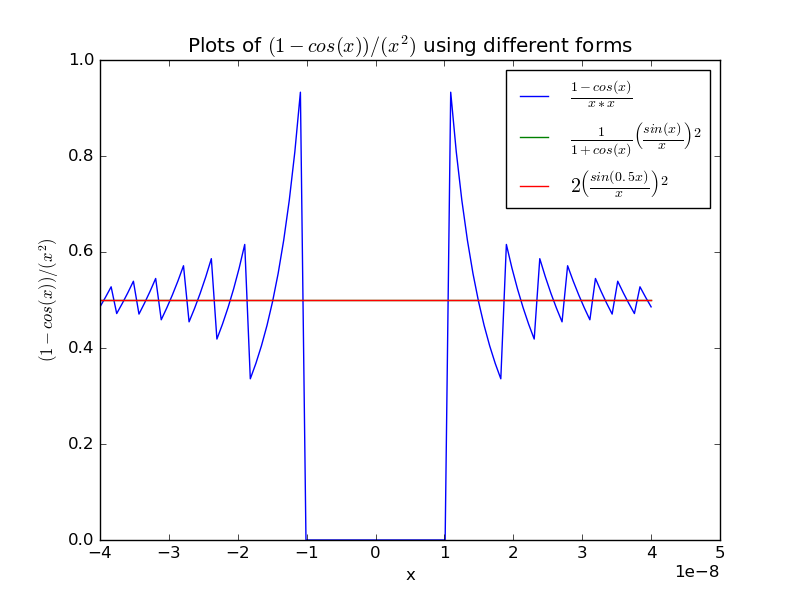
\includegraphics[width = \textwidth]{Q3.png}
 \caption{Graph of $(1 - cos(x))/(x^2)$ plotted using various methods}
 \label{fig:Q3}
\end{figure}

In the above figure we can see that the direct implementation of $(1 - cos(x))/(x*x)$ leads to incorrect results due to loosing
 of significant digits. The oscillations in this plot most probably arise due to rounding. We can see that both the above 
specified modifications of the functions lead to correct results.

\section{Question 4:}
\label{Question4}
The general methods for approximating $f(x)$ involve the use of Taylor series.
\begin{equation}
\label{eq:Forward}
 f(x+h) = \sum\limits_{k=0}^{\infty}\frac{f^{(k)}(x)}{k!}h^k
\end{equation}
\begin{equation}
\label{eq:back}
 f(x-h) = \sum\limits_{k=0}^{\infty}\frac{(-1)^kf^{(k)}(x)}{k!}h^k
\end{equation}

\subsection{First Order Approximation:}
\subsubsection{Forward difference}
Subtracting $f(x)$ from equation \ref{eq:Forward} we get:
\begin{equation*}
 f(x+h) - f(x) = hf'(x) + \left[\frac{h^2}{2!}f''(x) + \frac{h^3}{3!}f'''(x) ...\right]
\end{equation*}
which can also be written as
\begin{equation*}
 f(x+h) - f(x) = hf'(x) + \frac{h^2}{2}f''(\zeta)
\end{equation*}

\begin{equation}
\implies f'(x) = \frac{f(x+h)-f(x)}{h} - \left[ \frac{h}{2}f''(\zeta) \right]
\end{equation}
i.e first order approximation of $f'(x) = \mathlarger{\frac{f(x+h) - f(x)}{h}}$ and the error is $\left|\mathlarger
{\frac{h}{2}}f''(\zeta)\right|$
\subsubsection{Backward difference}
Subtracting equation \ref{eq:back} from $f(x)$ we get:
\begin{equation*}
 f(x) - f(x-h) = hf'(x) + \left[-\frac{h^2}{2!}f''(x) + \frac{h^3}{3!}f'''(x) ...\right]
\end{equation*}
which can also be written as
\begin{equation*}
 f(x) - f(x-h) = hf'(x) - \frac{h^2}{2}f''(\zeta)
\end{equation*}
\begin{equation}
\implies f'(x) = \frac{f(x)-f(x-h)}{h} + \left[\frac{h}{2}f''(\zeta) \right]
\end{equation}
i.e first order approximation of $f'(x) = \mathlarger{\frac{f(x) - f(x-h)}{h}}$ and the error is $\left|\mathlarger
{\frac{h}{2}}f''(\zeta)\right|$

\subsection{Second Order Approximation - Central difference}
Subtracting equation \ref{eq:back} from equation \ref{eq:Forward}, we get:
\begin{equation}
\label{eq:central}
 f(x+h) - f(x-h) = 2hf'(x) + \left[\frac{2h^3}{3!}f'''(x) + \frac{2h^5}{5!} ....\right]
\end{equation}
which can also be written as
\begin{equation*}
 f(x+h) - f(x-h) = 2hf'(x) + \frac{2h^3}{3!}f'''(\zeta)
\end{equation*}
\begin{equation}
 \implies f'(x) = \frac{f(x+h)-f(x-h)}{2h} +\left[-\frac{h^2}{6}f'''(\zeta)\right]
\end{equation}
Thus the second order approximation of $f'(x) = \mathlarger{\frac{f(x+h) - f(x-h)}{2h}}$ and the error is 
$\left|\mathlarger{\frac{h^2}{6}}f'''(\zeta)\right|$

\subsection{Fourth order approximation}
The fourth order approximation of $f'(x)$ can be derived from its second order approximation using Richardson's 
Extrapolation technique. Let us denote the central difference formula as $D(h)$ i.e
\begin{equation*}
 D(h) = \frac{f(x+h) - f(x-h)}{2h}
\end{equation*}
From equation \ref{eq:central} we have
\begin{equation}
\label{eq:4.1}
 f'(x) = D(h) - \frac{h^2}{3!}f^{(3)}(x) - \frac{h^4}{5!}f^{(5)}(x) ...
\end{equation}
We can also write $f'(x)$ for $2h$ in a similar way
\begin{equation}
\label{eq:4.2}
 f'(x) = D(2h) - 4\frac{h^2}{3!}f^{(3)}(x) - 16\frac{h^4}{5!}f^{(5)}(x) ...
\end{equation}
Multiplying equation \ref{eq:4.1} by 4 and subtracting from \ref{eq:4.2},
\begin{equation}
 3f'(x) = 4D(h) - D(2h) + 12\frac{h^4}{5!}f^{(5)}(x) ...
\end{equation}
Thus,
\begin{equation}
 f'(x) = \frac{4D(h) - D(2h)}{3} + 4\frac{h^4}{5!}f^{(5)}(x) ...
\end{equation}
\begin{equation}
 \implies f'(x) = \frac{-f(x+2h)+8f(x+h)-8f(x-h) + f(x-2h)}{12h} + O(h^4)
\end{equation}
Thus the fourth order approximation of \\$f'(x) = \mathlarger{\frac{-f(x+2h)+8f(x+h)-8f(x-h) + f(x-2h)}{12h}}$ and the 
error is $\left|4\frac{h^4}{5!}f^{(5)}(x)\right|$

\section{Question 5:}
\label{Question5}
In this question we analyze how the errors in the derivative of $sin(\pi/4)$ vary with changing value of $h$ using 
different finite difference schemes. We particularly analyze the finite difference schemes discussed in the previous 
question. Figure \ref{fig:Q5} shows the plots of the errors using the above schemes in logarithmic scales.
\begin{figure}[H]
 \centering
 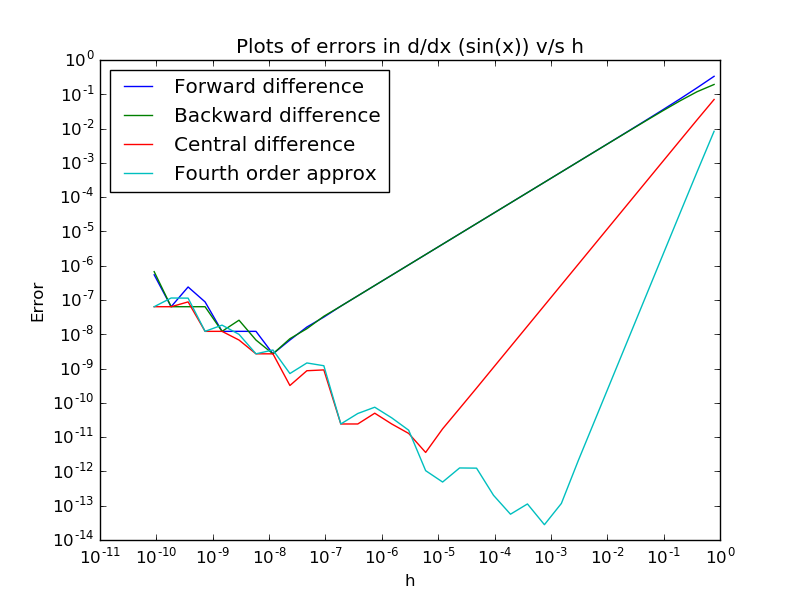
\includegraphics[width = \textwidth]{Q5.png}
 \caption{Errors in estimating $sin(\pi/4)$ using different difference schemes}
 \label{fig:Q5}
\end{figure}

From the above plot we can clearly see that: 
\begin{itemize}
 \item In case of forward and backward difference schemes $log(errors)$ vs $log(h)$  has slope roughly equal to $1$ 
 showing that $error \propto h$
 \item In case of central difference scheme $log(errors)$ vs $log(h)$ has a rough slope of $2$ showing that $error \propto
 h^2$
 \item In case of the 4th order approximation that we arrived at in the previous question $log(errors)$ vs $log(h)$ has
 a rough slope of $4$ showing that $error \propto h^4$
\end{itemize}

\section{Conclusion}

This assignment gives a better insight into floating point arithmetic, the risks involved in it and how to reduce the 
errors. The value of epsilon gives a better understanding of the system storage techniques and the data types used in C++.
Deriving the finite difference schemes for first derivative to $1^{st}$, $2^{nd}$ and $4^{th}$ orders of accuracy 
introduces different techniques that can be used to estimate a function to a better accuracy. The last question gave us a
visualization of the finite difference schemes and the errors involved in them. 

\end{document}

